\documentclass[12pt]{article}
\usepackage[paper=letterpaper,margin=1.5cm]{geometry}
\usepackage{amsmath}
\usepackage{amssymb}
\usepackage{amsfonts}
\usepackage{mathtools}
%\usepackage[utf8]{inputenc}
%\usepackage{newtxtext, newtxmath}
\usepackage{lmodern}     % set math font to Latin modern math
\usepackage[T1]{fontenc}
\renewcommand\rmdefault{ptm}
%\usepackage{enumitem}
\usepackage[shortlabels]{enumitem}
\usepackage{titling}
\usepackage{graphicx}
\usepackage[colorlinks=true]{hyperref}
\usepackage{setspace}
\usepackage{subfigure} 
\usepackage{braket}
\usepackage{color}
\usepackage{tabularx}
\usepackage[table]{xcolor}
\usepackage{listings}
\usepackage{mathrsfs}
\usepackage{stackengine}
\usepackage{physics}
\usepackage{afterpage}
\usepackage{pdfpages}
\usepackage[export]{adjustbox}
\usepackage{biblatex}

\setstackEOL{\\}

\definecolor{dkgreen}{rgb}{0,0.6,0}
\definecolor{gray}{rgb}{0.5,0.5,0.5}
\definecolor{mauve}{rgb}{0.58,0,0.82}


\lstset{frame=tb,
  language=Python,
  aboveskip=3mm,
  belowskip=3mm,
  showstringspaces=false,
  columns=flexible,
  basicstyle={\small\ttfamily},
  numbers=none,
  numberstyle=\tiny\color{gray},
  keywordstyle=\color{blue},
  commentstyle=\color{dkgreen},
  stringstyle=\color{mauve},
  breaklines=true,
  breakatwhitespace=true,
  tabsize=3
}
\setlength{\droptitle}{-6em}

\makeatletter
% we use \prefix@<level> only if it is defined
\renewcommand{\@seccntformat}[1]{%
  \ifcsname prefix@#1\endcsname
    \csname prefix@#1\endcsname
  \else
    \csname the#1\endcsname\quad
  \fi}
% define \prefix@section
\newcommand\prefix@section{}
\newcommand{\prefix@subsection}{}
\newcommand{\prefix@subsubsection}{}
\renewcommand{\thesubsection}{\arabic{subsection}}
\makeatother
\DeclareMathOperator*{\argmin}{argmin}
\newcommand{\partbreak}{\begin{center}\rule{17.5cm}{2pt}\end{center}}
\newcommand{\alignbreak}{\begin{center}\rule{15cm}{1pt}\end{center}}
\newcommand{\tightalignbreak}{\vspace{-5mm}\alignbreak\vspace{-5mm}}
\newcommand{\hop}{\vspace{1mm}}
\newcommand{\jump}{\vspace{5mm}}
\newcommand{\R}{\mathbb{R}}
\newcommand{\C}{\mathbb{C}}
\newcommand{\N}{\mathbb{N}}
\newcommand{\G}{\mathbb{G}}
\renewcommand{\S}{\mathbb{S}}
\newcommand{\bt}{\textbf}
\newcommand{\xdot}{\dot{x}}
\renewcommand{\star}{^{*}}
\newcommand{\ydot}{\dot{y}}
\newcommand{\lm}{\mathrm{\lambda}}
\renewcommand{\th}{\theta}
\newcommand{\id}{\mathbb{I}}
\newcommand{\si}{\Sigma}
\newcommand{\Si}{\si}
\newcommand{\inv}{^{-1}}
\newcommand{\T}{^\intercal}
\renewcommand{\tr}{\text{tr}}
\newcommand{\ep}{\varepsilon}
\newcommand{\ph}{\varphi}
%\renewcomand{\norm}[1]{\left\lVert#1\right\rVert}
\definecolor{cit}{rgb}{0.05,0.2,0.45}
\addtolength{\jot}{1em}
\newcommand{\solution}[1]{

\noindent{\color{cit}\textbf{Solution:} #1}}

\newcounter{tmpctr}
\newcommand\fancyRoman[1]{%
  \setcounter{tmpctr}{#1}%
  \setbox0=\hbox{\kern0.3pt\textsf{\Roman{tmpctr}}}%
  \setstackgap{S}{-.9pt}%
  \Shortstack{\rule{\dimexpr\wd0+.1ex}{.9pt}\\\copy0\\
              \rule{\dimexpr\wd0+.1ex}{.9pt}}%
}

\newcommand{\Id}{\fancyRoman{2}}

% Enter the specific assignment number and topic of that assignment below, and replace "Your Name" with your actual name.
\title{STAT 31020: Homework 6}
\author{Caleb Derrickson}
\date{February 21, 2024}

\begin{document}
\onehalfspacing
\maketitle
\allowdisplaybreaks

\tableofcontents

\newcommand{\scE}{\mathcal{E}}
\newcommand{\scL}{\mathcal{L}}
\newcommand{\scF}{\mathcal{F}}
\newcommand{\scJ}{\mathcal{J}}
\newpage
\section{Problem 1}
We will aim to prove the first-order optimality conditions Theorem 12.1 and Theorem 12.5 using two tools: the implicit function theorem (Theorem A.2) fo the case with equality constraints. That is, we aim to solve the problem
\begin{align*}
    &\min_{x \in \R^n} f(x)\\
    &\text{subject to } \ c_i(x) = 0, i \in \scE
\end{align*}
where the functions $f, c_i$ are smooth, and $\scE$ is a set of indices. A point which only satisfies the constraints is called \textit{feasible}. We aim to characterize the properties of a local minimum $x\star$, an extension of the first-order and second-order optimality conditions of unconstrained minimization. An important quantity used to express these conditions is called the Lagrangian,
\[\scL (x \lm) = f(x) - \sum_{i \in \scE} \lm_i c_i(x).\]
Here, the $\lm_i$'s are called the Lagrange multipliers. We will assume that at the solution $x\star$ we satisfy the linear independence constraint qualification LICQ. That is, we will assume that the set of vectors $\grad_i c_i(x\star), i \in \scE$ is linearly independent. I will call the matrix $J$ formed by  $\grad_i c_i(x\star), i \in \scE$ as rows, the Jacobian matrix. Therefore, we will assume $J$ to be full row rank. Observe one standard awkwardness optimization notation standard; gradients of individual functions are thought of as columns but if you look at the definition of the Jacobian they would be 
thought of as rows. This may affect you as you interpret the implicit function theorem.

\newpage
\subsection{Problem 1, part 1}
Use the implicit function theorem to show that, for equality constraint problems you have a partition of the unknown vector $x = (x_1, x_2)$ such that the dimension of $x_2$ equals the number of constraints in $\scE$. Show that there is a function $h(x_1)$ such that $c_i(x_1, h(x_1)) = 0, i \in \scE$ (you can assume it is as differentiable as $c_i$ is) for some neighborhood of $x_1\star$. Use the implicit function theorem to compute its Jacobian and connect it with the constraint Jacobian $J$. State the relationship between the equality constrained problem and the unconstrained problem $\min_{x_1} f(x_1, h(x_1))$ in the same neighborhood of $x\star$.
\partbreak
\begin{solution}

    For clarity, I will provide the Implicit function below, which is from its Wikipedia page:
      \begin{center}\rule{17cm}{0.1mm}\end{center}
    \begin{quote}
    \vspace{-5mm}
        \underline{The Implicit Function Theorem.}

        Let $f: \R^{m+n} \into \R^m$ be a continuously differentiable function, and let $\R^{m + n}$ have coordinates $(x_1, x_2)$. Fix a point $(x_1\star, x_2\star) = (x_1\star)_{\R^n} \oplus (x_2\star)_{\R^m}$ with $f(x_1\star, x_2\star) = 0$, where $0 \in \R^n$. If the Jacobian matrix
        \[\scJ_{f, x_2} = \mqty[\frac{\partial f_i}{\partial x_{2, j}}(x_1\star, x_2\star)]\]
        is invertible, then there exists an open set $U \subset \R^n$ containing $x_1\star$ such that there exists a unique continuously differentiable function $h: U\into \R^m$ such that $h(x_1) = x_2$, and $f(x_1, h(x_1)) = 0$ for all $x \in U$. Moreover, if we have 
        \[\scJ_{f, x_1}(x_1\star, x_2\star) = \mqty[\frac{\partial f_i}{\partial x_{1, j}}(x_1\star, x_2\star)],\]
        then we can write the Jacobian matrix of partial derivatives of $h$ in $U$ as 
        \[\mqty[\frac{\partial h}{\partial x_{1, j}}(x)] = -\mqty[\scJ_{f, x_2}(x, h(x))]\inv \mqty[\scJ_{f, x_1}(x, h(x))]\]
    \vspace{-15mm}
    \end{quote}
    \begin{center}\rule{17cm}{0.1mm}\end{center}
    I have \textit{partially} applied the notation from the Wikipedia page to our notation, where the only critical piece left out is our choice of $f(x)$. The most obvious choice would be the constraint equalities, $c_i(x)$, but in what form is somewhat up to interpretation. Due to our convention of taking Jacobians as rows of the partial derivatives, then our choice of 
    \[F(x) = \mqty[c_1(x)\\c_2(x)\\\vdots\\c_m(x)]\]
    makes the most reasonable choice. By the given partition, we choose $x_2 \in \R^m$ to be the associated values to the constraints. By this reasoning, we have that $x_1 \in \R^n$. The Jacobian of $F$, which we will denote by $\scJ$, will then be 
    \[\grad_x F (x) = \scJ = \mqty[\grad_x c_1(x_1, x_2)\\\vdots\\ \grad_x c_m(x_1, x_2)] = \mqty[\grad_{x_1} c_1(x_1, x_2) & \grad_{x_2} c_1(x_1, x_2)\\\vdots&\vdots\\ \grad_{x_1} c_m(x_1, x_2) & \grad_{x_2} c_m(x_1, x_2)] = \begin{array}{c|c}
        \big[\scJ_{F, x_1}(x_1, x_2) & \scJ_{F, x_2}(x_1, x_2)\big]
    \end{array}\]
    Since we suppose that LICQ holds, then we would have that $\scJ_{F, x_2}(x_1, x_2)$ is an $m \times m$ matrix with lineraly independent columns. This would then mean that $\scJ_{F, x_2}(x_1, x_2)$ is invertible. Note that at the minimum, $(x_1\star, x_2\star)$ the equality constraints will obviously hold, so that $F(x_1\star, x_2\star) = 0$. Therefore, by the Implicit Function Theorem, there exists an open set $U \subset \R^n$, containing $x_1\star$, for which there is a unique continuously differentiable function $h: U \into \R^m$ such that $h(x_1) = x_2$ and $F(x_1, h(x_1)) = 0$, for all $x_1 \in U$. By construction of the function $F$, we have that $c_i(x_1, h(x_1)) = 0 $ for all $i \in \scE$. This then shows the first part of this part. We next need to apply the Implicit Function Theorem's implication on the gradient of $h$. We have that 
    \[\mqty[\frac{\partial h}{\partial x_{1, j}}(x)] = -\mqty[\scJ_{f, x_2}(x, h(x))]\inv \mqty[\scJ_{f, x_1}(x, h(x))]\] 
    By taking the gradient of our function $F$, we have that
    \[\grad_x \left(F(x_1, h(x_1))\right) = \left( \grad_xF(x_1, h(x_1)\right)\T \grad_x h(x_1).\]
    This then implies
    \[\grad_x F(x_1, h(x_1)) =  -\left( \grad_xF(x_1, h(x_1)\right)\T \mqty[\scJ_{f, x_2}(x, h(x))]\inv \mqty[\scJ_{f, x_1}(x, h(x))]\]
    For the sake of simplicity, I will denote the separate terms as the variable in which we are differentiating. So the term inverse term will just be expressed as $x_2\inv$. Then the transposed gradient, with taking gradient with respect to $x_1$ and $x_2$, will be written as 
    \[x\T = \mqty[x_1\T \\x_2\T].\]
    Therefore, we have 
    \[\grad_x F(x_1, h(x_1)) = \mqty[x_1\T \\x_2\T] \mqty[-x_2]\inv \mqty[x_1] = \mqty[-x_1\T x_2\inv x_1\\-x_2\T x_2\inv x_1] = \mqty[-x_1\T x_2\inv \\-x_2\T x_2\inv]\mqty[x_1]\]
    I can assure you that all matrix multiplications are correct, since the matrix associated with $x_1$ and $x_2$ are $m \times n$ and $m \times m$, respectively. This can be inferred by my entire writing of the Jacobian at the top of this page. This equality will hold only in our open set $U$, by the Implicit Function Theorem.
\end{solution}
\newpage
\subsection{Problem 1, part 2}
Write the first-order optimality conditions for $\min_{x_1} f(x_1, h(x_1))$ at $x_1\star$ and infer from here the \textit{first-order optimality conditions for equality constrained optimization} of Theorem 12.1. If you look carefully at them it should be pretty clear what the Lagrange multipliers should be; particularly if you take a look at what you are supposed to obtain (to figure the answer out you can work backwards from what you try to obtain by obtaining the Lagrange multipliers from the optimality 
conditions). We will call these Lagrange multipliers sometimes the optimal Lagrange multipliers (since they satisfy the KKT conditions), and we will denote them by $\lm_i\star, i \in \scE$.
\partbreak
\begin{solution}

    By the KKT conditions, since we are working only with equality conditions, we have only three implications (assuming there exists some $\lm\star$), 
    \begin{align*}
        \grad_x \scL(x\star, \lm\star) &= 0,\\
        c_i(x\star) &= 0,  \quad \forall \ i \in \scE\\
        \lm_i\star c_i(x\star) &= 0 \ \ \quad \forall \ i \in \scE
    \end{align*}
    By the form of the Jacobian given, we can see that $\lm = \grad_{x_1}h(x_1)$. This has a value at the minimum $x_1\star$, which is $\lm\star = \grad_{x_1}h(x_1\star)$. Here the Lagrangian of the system is with respect to our new minimization problem $\min_{x_1} f(x_1, h(x_1))$, which from the terminology in the first part, is $F$. Therefore, the gradient of the Lagrangian is given as 
    \[\grad_x \scL(x\star, \lm\star) = \grad_x \left( F - \sum_{i \in \scE} \lm_i\star \grad c_i(x\star)\right) \implies \grad_x F = \sum_{i \in \scE} \lm_i\star \grad^2c_i(x\star) \]
\end{solution}

\newpage
\subsection{Problem 1, part 3}
As we learned in class, we call in this case the feasible directions cone at a feasible point the set $\scF(x) = \{ d \in \R^n : \grad_x c_i(x)\T d = 0, i \in \scE\}$, and we also learned that, under LICQ at $x$, for any $d \in F(x)$ we have a feasible arc $\Tilde{x}(t): \scN(0) \into \R^n$ originating at $x$ and whose tangent at zero is $d$. That is, 
\[\Tilde{x}(0) = x, \quad \frac{d}{dt}\Tilde{x}(t) \Big|_{t = 0} = d, \quad c_i(\Tilde{x}(t)) = 0,  \quad \forall \ i \in \scE, \ \forall t \in \scN(0)\]
Here $\scN(0)$ is an open neighborhood of zero on the real axis. We can assume that this arc has the same differentiability class as the data functions themselves (this is a consequence of the implicit theorem). We denote the second derivative at zero for this arc to be 
\[w := \frac{d^2}{dt^2}\Tilde{x}(t)\Big|_{t = 0}\]
Use the chain rule twice on the equation stating the feasibility of the arc to prove that
\[\grad_x c_i(x)\T w + d\T \grad_{xx}^2c_i(x) d = 0, \ \forall \ i \in \scE\]
\partbreak
\begin{solution}
    
    We will begin calculations:
    \tightalignbreak
    \begin{align*}
        &c_i(\Tilde{x}(t)) = 0 &\text{(Given.)}\\
        \implies &\grad\left( c_i\Tilde{x}(t)\right) = 0 &\text{(Taking derivative.)}\\
        =& \grad c_i(\Tilde{x}(t))\T \frac{d}{dt}\Tilde{x}(t) = 0 &\text{(Chain rule.)}\\
        \implies & \grad^2(c_i) = \grad\left(\grad c_i(\Tilde{x}(t))\T \frac{d}{dt}\Tilde{x}(t) \right) = 0 &\text{(Taking second derivative.)}\\
        =& \left(\grad^2_{xx} c_i(\Tilde{x}(t)) \frac{d}{dt}\Tilde{x}(t)\right)\T \frac{d}{dt}\Tilde{x}(t) + \grad_x c_i(\Tilde{x}(t))\T \frac{d^2}{dt^2}\Tilde{x}(t) &\text{(Product rule.)}\\
        =&\left(\frac{d}{dt}\Tilde{x}(t)\right)\grad^2_{xx} c_i(\Tilde{x}(t))\T  \left(\frac{d}{dt}\Tilde{x}(t)\right) + \grad_x c_i(\Tilde{x}(t))\T \frac{d^2}{dt^2}\Tilde{x}(t) &\text{(Rearranging.)}\\
        \implies & d\T \grad_{xx}^2c_i(x)d + \grad_x c_i(x)\T w = 0 &\text{(Evaluating at $t = 0$.)}
    \end{align*}\vspace{-12mm}\alignbreak
\end{solution}
\newpage
\subsection{Problem 1, part 4}
Assume now that the arc defined at point (3) originates at the solution $x\star$ of the problem and consider the Lagrange multipliers from point (2). Prove that
\[\frac{d^2}{dt^2}f(\Tilde{x}(t)) \Big|_{t = 0} = d\T \grad_{xx}^2 \scL (x\star, \lm\star)\T d\]
\partbreak
\begin{solution}

    We first start with taking the second gradient of the Lagrangian. For the sake of simplicity, we will write $\Tilde{x}$ as $x$, and clearly specify when necessary. From the form given, we see
    \begin{align*}
        \scL &= f(x) - \sum_{i \in \scE} \lm_i c_i(x) \\
        \grad_x \scL &= \grad_x f(x) - \sum_{i \in \scE} \lm_i \grad_x c_i(x)\\
        \grad_{xx}^2 \scL &= \grad_{xx}^2 f(x) - \sum_{i \in \scE} \lm_i \grad_{xx}^2 c_i(x)
    \end{align*}
    Where the left hand side is of the form below:
    \tightalignbreak
    \begin{align*}
        \frac{d}{dt}\left[ f(\Tilde{x}(t)\right] &= \grad f(\Tilde{x}(t)) \T \frac{d}{dt}\Tilde{x}(t)\\
        \frac{d^2}{dt^2}\left[ f(\Tilde{x}(t) \right] &= \left( \grad^2_{xx} f(\Tilde{x}(t)) \frac{d}{dt}\Tilde{x}(t)\right)\T \frac{d}{dt}\Tilde{x}(t) + \grad_{x} f(\Tilde{x}(t))\T \frac{d^2}{dt^2}\Tilde{x}(t)\\
        &= \left(\frac{d}{dt}\Tilde{x}(t)\right)\T \grad^2_{xx} f(\Tilde{x}(t))\T \frac{d}{dt}\Tilde{x}(t) + \grad_{x} f(\Tilde{x}(t))\T \frac{d^2}{dt^2}\Tilde{x}(t)
    \end{align*}
    \vspace{-12mm}\alignbreak
    Then, when evaluating,
    \[\frac{d^2}{dt^2}f(x)\Big|_{t=0} = d\T \grad^2_{xx} f(x\star)\T d + \grad_x f(x\star)\T w\]
    By the KKT Theorem assumed, we have that the gradient of the Lagrangian is zero (at the optimal point $x\star, \lm\star)$. Therefore, we can replace the gradient of the function with the summation shown above. Then,
    \[\frac{d^2}{dt^2}f(x)\Big|_{t=0} = d\T \grad^2_{xx} f(x\star)\T d + \left(\sum_{i \in \scE} \lm_i\star \grad c_i(x\star)\right)\T w\]
    But by problem 3, we can replace the gradient of the constraint with its second, for some $d$ in the feasible set. We finally then have that
    \[\frac{d^2}{dt^2}f(x)\Big|_{t=0} = d\T \grad_{xx}^2f(x\star)d - \sum_{i \in \scE} \lm_i\star d\T \grad_{xx}^2 c_i(x\star)d = d\T \scL(x\star, \lm\star)d\]
\end{solution}

\newpage
\subsection{Problem 1, part 5}
Use now the fact that 0 is a minimum point of the problem $\min_{i} f(\Tilde{x}(t))$ for the arc defined at part (4) to prove the second-order optimality conditions of Theorem 12.5 for problems with equality constraints starting from the ones for unconstrained optimization.
\partbreak
\begin{solution}

    Since $t = 0$ is now a minimum of the unconstrained solution, from part 4, we have that the second derivative of $f$ is equivalent to the Hessian of the Lagrangian (evaluated with respect to $d\T$ and $d$). From Theorem 12.5, the second order sufficient conditions, we need to show that 
    \[w\T \grad^2_{xx}\scL (x\star, \lm\star)\T w \geq 0, \quad \text{ for all } w \in C(x\star, \lm\star).\]
    By 12.53 in the text, for equality constraints only, the critical cone is equivalent to 
    \[C(x\star, \lm\star) = \{ w \in \scF(x\star) : \grad c_i(x\star)w = 0\}.\]
    By the way we've defined the feasible set, then immediately the feasible set is equal to the convex cone. Therefore, we don't have to worry about the domains of $d$. Since $x\star$ is a local minimum, by the second order sufficient conditions $\frac{d^2}{dt^2}f(x\star) > 0$, within some neighborhood of $x\star$. Therefore the second order sufficient conditions has been satisfied. 
\end{solution}

\newpage
\subsection{Problem 1, part 6}
Assume now slightly stronger conditions than the ones at point (5) (which is what we will assume for almost all optimization problems when looking at algorithms). That is, assume that there exist $\sigma > 0$ such that
\[d \in F(x\star) \implies d\T \grad^2_{xx}\scL(x\star, \lm\star)\T d \geq \sigma\norm{d}^2\]
Prove that the following matrix is invertible
\[\mqty[\grad^2_{xx}\scL(x\star, \lm\star) &J\T\\ J&0]\]
\partbreak
\begin{solution}

    Denote the given matrix by $A$ for simplicity. Here, let's suppose false. That is, there exists an $\textbf{x} \neq 0$, but $\textbf{x} \in \ker (A)$. Then $A\textbf{x} = \textbf{0}$. Since the given matrix is of finite size, we can write $\textbf{x} = [\textbf{x}_1, \textbf{x}_2]$ of suitable dimensions. Thus, 
    \[A\textbf{x} = \mqty[\grad^2_{xx}\scL(x\star, \lm\star) &J\T\\ J&0]\mqty[\textbf{x}_1\\\textbf{x}_2] \implies \mqty[\grad^2_{xx}\scL(x\star, \lm\star)\textbf{x}_1 + J\T \textbf{x}_2\\ J\textbf{x}_1] = \mqty[0\\0].\]
    Since we have that the Jacobian is invertible (it has full column rank by LICQ), then $J\textbf{x}_1 = 0 \iff \textbf{x}_1 = 0$. Plugging that into the first equation, we have that $J\T \textbf{x}_2 = 0$, but since $J\T$ is invertible (the eigenvalues of the matrix remain constant under transposition, assuming over the real numbers), then $J\T \textbf{x}_2 = 0 \iff \textbf{x}_2 = 0$. Then, $\textbf{x} = \textbf{x}_1 \oplus \textbf{x}_2 = 0 \oplus 0 = 0$. But we assumed that $\textbf{x} \neq 0$, which leads to a contradiction. Therefore, the only element in the kernel of $A$ is the zero vector, implying that $A$ is invertible.  
\end{solution}

\newpage
\subsection{Problem 1, part 7}
Observe that the first-order KKT conditions at part 2 are nonlinear equations in this case. Write the Newton iteration for them and explain what is the significance of the finding in part 6. 
\partbreak
\begin{solution}

    For multivariable systems, the Newton's method for root finding is given as 
    \[\textbf{x}_{n+1} = \textbf{x}_n - J_\textbf{F}(\textbf{x}_n)\inv F(\textbf{x}_n)\]
\end{solution}

\newpage
\section{Problem 2}
Create a set of random linear programs in standard form as follows:
\begin{itemize}
    \item Set the random number generator seed at a prescribed value "s".
    \item Create a matrix A of size (m, n) with random standard normal entries.
    \item Let $e = (1, 1, ..., 1, 0, 0, ..., 0)\T , e \in \R^n$. Here the first m components of $e$ are equal to one. Compute $b = Ae$.
    \item Create now a random objective as follows: $c = (1, 1, ..., 1)\T + 50 \times u$; here $u\in \R^n$ is a random vector for which each component is independently uniformly distributed in $(0, 1)$.
\end{itemize}
Read Section 13.3 and Implement the simplex algorithm (Procedure 13.1 , with the pivoting rules are described in Section 13.3 ) starting from the basic feasible point. Apply the simplex method for n=2m, at 10 random instances and report the mean and standard deviation of the time it took to solve the problem; if you encounter degeneracy (exact ties when determining leaving variables; extremely unlikely), then remove that example from the statistic, but report that you have encountered it. Do it for m=5,10, $..., $ for as high as your computation is tolerable on your computer (overall run time for this exercise should not be more than 1 hour, but how large of a size you can afford is a function of your platform; whether it is private or shared, etc).
\partbreak
\begin{solution}

    I will provide the graphs of average time, standard deviation below. I am not reporting a plot of degeneracy, since I did not encounter any. For the simplex method, I ran it up to size $m = 2000$, with step 5, and allowed 100 loops of the simplex algorithm. We see, as expected, that the average time to compute simplex method increases at a steady pace for increasing dimensions. Also, the variance in time seems to be stable, relatively. Since the higher dimensions would just have more computation, it seems reasonable that the variance would have greater spikes. There does seem to be a general increasing trend, however. 
\end{solution}

\begin{figure}[!h]
    \centering
    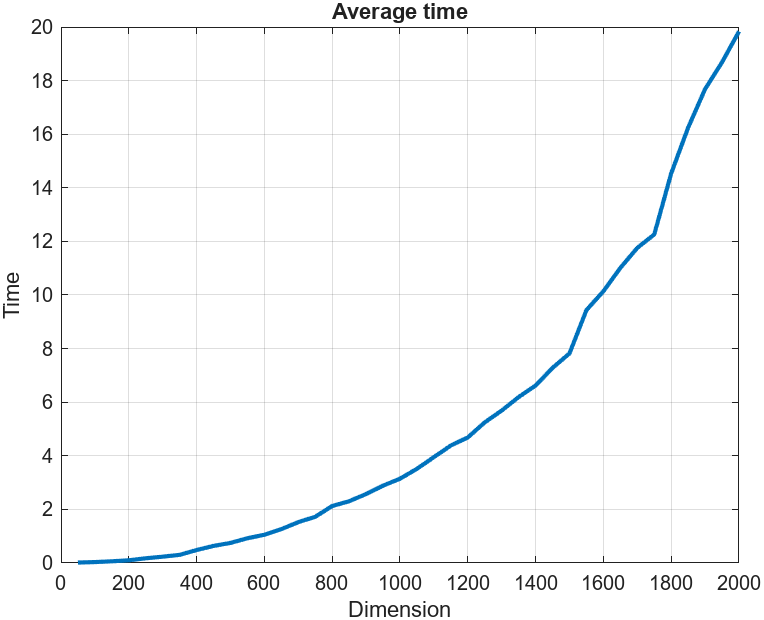
\includegraphics[width = 0.6\textwidth]{Figures/Average_time.png}
    \caption{Average time for Simplex method to act on a random matrix of variable size.}
    \label{fig:avg_time}
\end{figure}

\begin{figure}[!h]
    \centering
    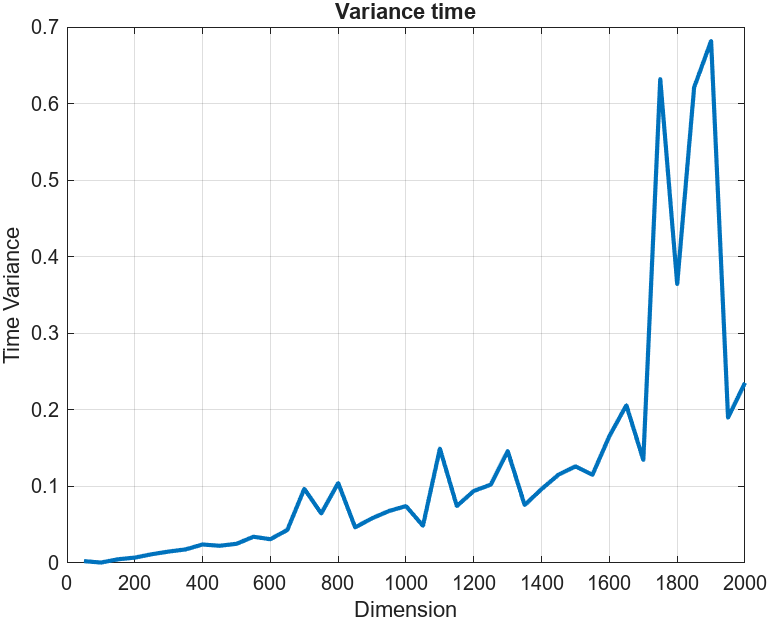
\includegraphics[width = 0.6\textwidth]{Figures/Variance.png}
    \caption{Associated variance for Problem 2.}
    \label{fig:variance}
\end{figure}

\end{document}